\subsection{Standard algorithm}

We first introduce our problem formally.

\begin{problem}[$\mathbb F_2$-PersBarcodes]
  Instance: let $\mathbb K$ be a maximal (finite) filtered simplicial complex. \\
  Question: compute $\Pers(H_*(\mathbb K; \mathbb F_2))$.
\end{problem}

Let $K$ be a finite simplicial complex and $\mathbb K = \{K_i\}_{i=0}^n$ be a maximal filtration of $K$. Let $\sigma_1, \ldots, \sigma_n$ be the (unique) ordering of the simplices of $K$ induced by $\mathbb K$.

We consider the simplicial chain complex of $K$ with coefficients in $\mathbb F_2$: $C(K; \mathbb F_2) = \{(\restr Ki, \partial_i)\}_{i=0}^{\dim K}$. Let $n_i = \left\lvert \restr Ki \right\rvert$. By picking canonical bases for each $\restr Ki$, we may represent $\partial_i$ as a $n_{i-1} \times n_{i}$ matrix with entries in $\mathbb F_2$ for each $i \geq 1$. We combine the boundary maps of each chain group into a single map, $\partial: \bigoplus_{i=0}^{\dim K} C_i \to \bigoplus_{i=0}^{\dim K} C_i$. To do this, we pick our basis as the simplex ordering $\sigma_1, \ldots, \sigma_n$ and let $\partial$ be a $n \times n$ matrix defined by
\[
  \partial[i,j] = \begin{cases}
    1 & \text{if $\sigma_i$ is a face of $\sigma_j$}, \\
    0 & \text{otherwise}.
  \end{cases}
\]
This map agrees with the boundary maps $\partial_i$ of the simplicial chain complex, and $\partial$ is strictly upper triangular. We call $\partial$ the \emph{boundary matrix} of $\mathbb K$.

\begin{figure}
  \centering
  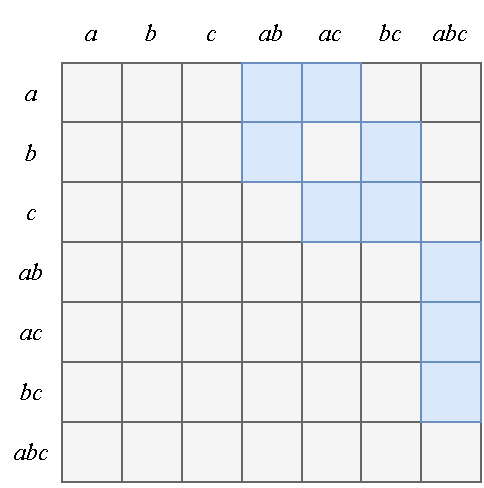
\includegraphics[width=0.5\textwidth]{content/4-comp-top/images/boundary-ex}
  \caption{The boundary matrix for the simplex ordering $(a, b, c, ab, ac, bc, abc)$. A grey cell corresponds to a 0, and a blue cell corresponds to a 1.}
  \label{fig:boundary-ex}
\end{figure}

\begin{example}
  Figure \ref{fig:boundary-ex} is a visualisation the boundary matrix for the simplex ordering $(a, b, c, ab, ac, bc, abc)$.
\end{example}

The prevalent method for solving \textsc{$\mathbb F_2$-PersBarcodes} this problem is matrix reduction (effectively a variant of the Smith normal form algorithm). We let $M \in M_n(\mathbb F_2)$ and define $\low_M(i) = \max\{j: M[i, j] \neq 0\}$; that is, $\low(i)$ is the largest row index of a non-zero entry in column $i$ (we let it take some sentinel value otherwise). A column operation of the form $M_i \gets M_i + M_j$ is called \emph{reducing} if $j < i$ and $\low_M(i) = \low_M(j)$. A matrix is called \emph{reduced} if no more reducing operations can be performed on it. A matrix $R$ is a \emph{reduction} of $M$ if $R$ is reduced and arises from a sequence of reducing operations from $M$.

\begin{lemma}
  \label{lem:reduction-correct}
  Let $K$ be a finite simplicial complex and $\mathbb K = (K_i)_{i=0}^m$ be a filtration of $K$, such that $K_m = K$. Let $\partial$ be the boundary matrix of $\mathbb K$ (with basis some ordering of the simplices compatible with $\mathbb K$) and $R$ a reduction of $\partial$. Then $(i, j) \in \Pers(\mathbb K)$ if and only if
  \begin{enumerate}
    \item $j \neq \infty$ and $\low_R(j) = i$;
    \item $j = \infty$ and $\low^{-1}_R(i) = \varnothing$. 
  \end{enumerate}
\end{lemma}

\begin{proof}
  We can consider the reduction algorithm as a variant of a Smith normal form algorithm (although the reduction matrix is not quite in Smith normal form), and so by the structure we gave the persistence module in Section \ref{ssec:pers_modules} we see that the reduction algorithm indeed gives us the persistent barcodes as above.
\end{proof}

Lemma \ref{lem:reduction-correct} shows us that it is sufficient to find a reduction of the boundary matrix to compute the persistent barcodes. 

Before looking at methods for computing the reduction, we look at how to read off the persistent barcodes. We split $\Pers(H_*(\mathbb K))$ into two sets:
\[ \Pers(H_*(\mathbb K)) = \Pers_0(H_*(\mathbb K)) \cup \Pers_\infty(H_*(\mathbb K))\]
where $\Pers_0(H_*(\mathbb K))$ comprises of the finite intervals $(i,j)$ and $\Pers_\infty(H_*(\mathbb K))$ comprises of the infinite intervals $(i, \infty)$. We can compute $\Pers_0(\mathbb K)$ by iterating over each $j \in \{1, \ldots, n\}$ and computing $\low_\partial(j) = i$, which forms $(i, j) \in \Pers_0(\mathbb K)$. For $\Pers_\infty(H_*(\mathbb K))$, we just note the $i \in \{1, \ldots, n\}$ that does not have a corresponding $j > i$ such that $\low_\partial(j) = i$. The running time of this interpretation depends on the implementation of the $\low$ function; for example, using a hash table gives us a constant time evaluation and $O(n)$ time to update after a column operation, which would give us a constant time interpretation. 

We now introduce the problem of finding the reduction of $\partial$. 

\begin{problem}[$\mathbb F_2$-PersReduction]
  Instance: let $\partial$ be the boundary matrix of some maximal filtered simplicial complex. \\
  Question: compute a reduction $R$ of $\partial$.
\end{problem}

\begin{algorithm}
  \caption{The standard reduction algorithm for \textsc{$\mathbb F_2$-\-Pers\-Reduc\-tion}.}
  \label{alg:std-reduction}
  \begin{algorithmic}[1]
      \Function{Low}{$n \times n$ matrix $R$, $i \in \{1, \ldots, n\}$}
        \State\Return lowest non-zero entry of column $i$
      \EndFunction
      \Function{IsColReduced}{$n \times n$ matrix $R$, $i \in \{1, \ldots, n\}$}
        \State\Return whether there is $i' < i$ such that $\Call{Low}{R, i'} = \Call{Low}{R, i}$
      \EndFunction
      \Function{StdReduction}{$n \times n$ boundary matrix $\partial$}
        \State $R \gets \partial$
        \For{$i \gets 1$ to $n$}
          \While{not \Call{IsColReduced}{$R, i$}}
            \For{$j=1$ to $i$}
              \If{$\Call{Low}{R, i} = \Call{Low}{R, j}$}
                \State add column $j$ to $i$ and break for loop
              \EndIf
            \EndFor
          \EndWhile
        \EndFor
        \State\Return $R$
      \EndFunction
  \end{algorithmic}
\end{algorithm}

Algorithm \ref{alg:std-reduction} is the standard reduction algorithm for persistent homology, first introduced by \textcite{edelsbrunner2000topological}. We will refer to this algorithm as \textsc{S}.

The running time of Algorithm \ref{alg:std-reduction} is $O(n^3)$ as
\begin{enumerate}
  \item adding a column to another column runs in $O(n)$ time; and
  \item calling the function $\textsc{Low}$ can be achieve in $O(1)$ time using a hash table, this hash table can be updated in $O(n)$ for each column operation.
\end{enumerate}

We are clear on the correctness of such a reduction, if the algorithm terminates then it is clear we meet the requirements of $R$ being a reduction. But we must prove that Algorithm \ref{alg:std-reduction} terminates. On to the main loop (line \texttt{9} onwards), we first claim that this terminates. Although not immediately obvious, we assert that $\textsc{IsColReduced}(i)$ will evaluate true by repeating \texttt{11} to \texttt{15}. Trivially, $\textsc{IsColReduced}(1)$ is always true. We now let $i > 1$ and assume that $\textsc{IsColReduced}(j)$ is true for each $j \in \{1, \ldots i\}$. As $\textsc{IsColReduced}(i)$ is false, there is $i_1 < i$ such that $\textsc{Low}(i_1) = \textsc{Low}(i)$. So we add the $i_1$th column to the $i$th column, making the new value of $\textsc{Low}(i)$ strictly less than $\textsc{Low}(i_1)$ (as, by definition, every entry below $\textsc{Low}(i_1)$ is zero). To appreciate this, we recall that we are in $\mathbb F_2$. If $\textsc{IsColReduced}(i)$ is true, we are done; otherwise, there is $i_2 < i$ such that $\textsc{Low}(i_2) = \textsc{Low}(i) < \textsc{Low}(i_1)$. Again, we perform the appropriate column operation. We continue this operation, and as there are only a finite number of rows (that is, a finite number of unique values for \textsc{Low}), then we must reach a point at which $\textsc{IsColReduced}(i)$ is false. The final conclusion is clear by induction. 


% First, we learn to read the ranks of the homology groups of $K$. Let $R \in M_m(\mathbb F_2)$ be the resulting matrix from running the standard algorithm described above on $\partial$. Define
% \begin{align*}
%   \operatorname{zeros}_p(R) & = \left\{
%   i: \text{column $i$ in $R$ is zero and $\dim\sigma_i=p$}
%   \right\},                             \\
%   \operatorname{lows}_p(R)  & = \left\{
%   i: \text{$\operatorname{low}(j) = i$ for some $j$ and $\dim\sigma_i=p$}
%   \right\}.
% \end{align*}
% If $K_i = \{\sigma_j\}_{j=1}^i$, we claim that $\operatorname{zeros}_p(R) - \operatorname{lows}_p(R) = \beta_p$, which can be seen by observing that $\operatorname{zeros}_p(R)$ is the rank of the $p$-cycles, and $\operatorname{lows}_p(R)$ is the rank of the $p$-boundaries.

% Next, we move to persistent homology. Let $f: K \to \R$ be defined on our simplicial complex as in the last section which induces our filtration, with associated sequence $\{a_i\}_{i=0}^m$. If $K_i = \{\sigma_j\}_{j=1}^i$ then $(a_i, a_j) \in \dgm_p(f)$ if and only if $i = \operatorname{low}(j)$ and $\dim\sigma_i = p$. Now we assume otherwise, so there is a step in the filtration in which more than one simplex is added. We simply construct the filtration $\{K_i'\}_{i=0}^m$ such that $K_i' =  \{\sigma_j\}_{j=1}^i$ and let $k': \Z_{\geq 0} \to \Z_{\geq 0}$ be the sequence such that $K_i = K'_{k'(i)}$ for all $i$. Now define $k: \Z_{\geq 0} \to \Z_{\geq 0}$ as $i \mapsto \min\{i': k(i') \geq i \}$. This is a mapping between our filtration and a filtration which only adds one simplex at a time when we move up. Let $(i, j)$ be the indices of some point in the $p$th persistence diagram for $K'$. Then $(a_{k(i)}, a_{k(j)}) \in \dgm_p(f)$
